\documentclass[table,aspectratio=43,mathserif,xcolor={usenames,dvipsnames,svgnames,table},10pt]{beamer}

\usetheme[titleformat frame=smallcaps]{metropolis}
\usepackage{appendixnumberbeamer}
\usepackage{booktabs}
\usepackage[utf8]{inputenc}

\usepackage{graphicx}
\usepackage{multimedia}

\usepackage{tikz}
\usetikzlibrary{arrows}
% \usetikzlibrary{arrows.meta}
\usetikzlibrary{positioning,calc}
\usetikzlibrary{decorations.pathreplacing}
\usetikzlibrary{decorations.markings}
\usetikzlibrary{fit}
\usetikzlibrary{shapes.callouts}
\usetikzlibrary{shapes.geometric}
\usetikzlibrary{matrix}
\usetikzlibrary{spy}
\setbeamertemplate{caption}{\raggedright\insertcaption\par}
\renewcommand{\footnotesize}{\tiny}
\newcommand{\norm}[1]{\left\lVert #1 \right\rVert}
\def\doubleunderline#1{\underline{\underline{#1}}}
\usepackage{animate}
\usepackage{svg}
\beamertemplatenavigationsymbolsempty

\tikzset{
  big arrow/.style={
    decoration={markings,mark=at position 1 with {\arrow[scale=1.4]{latex}}},
    postaction={decorate},
    shorten >=2.5pt}}
\tikzset{
  big 2arrow/.style={
    decoration={markings,mark=at position 0 with {\arrow[scale=-1.4]{latex}},mark=at position 1 with {\arrow[scale=1.4]{latex}}},
    postaction={decorate},
    shorten >=2.5pt}}

\tikzset{onslide/.code args={<#1>#2}{%
  \only<#1>{\pgfkeysalso{#2}} % \pgfkeysalso doesn't change the path
}}

\pgfdeclarelayer{background}
\pgfdeclarelayer{foreground}
\pgfsetlayers{background,main,foreground}

% 
\usepackage[style=numeric,natbib]{biblatex}
\addbibresource{references.bib}

\title[NMT]{Neural Machine Translation}
\author[Arul Selvam Periyasamy]{Arul Selvam Periyasamy}
\institute[University of Bonn]{Rheinische Friedrich-Wilhelms-Universit\"at Bonn\\
Seminar: Natural Language Processing}

\date{\today}
% \logo{\includegraphics[width=2.5cm]{images/ais_uni_logo.eps}}

\begin{document}

\maketitle


\begin{frame}{Agenda}
 \begin{itemize}
  \item<+-> Introduction to Machine Translation
  \item<+-> Evaluation Metric
  \item<+-> Statistical Phrase-Based Translation
  \item<+-> Introduction to Deep Learning
  \item<+-> Neural Machine Translation

 \end{itemize}
\end{frame}

\begin{frame}{Motivation}
\begin{itemize}
 \item<+-> Translation: The process of translating words or text from one language into another (OED).
 \item<+-> Machine Translation: Translation carried out by a computer (OED).
 \item<+-> Why do we need it?
 \item<+-> Do I need to convince that we need machine translation?
\end{itemize}
\end{frame}


\begin{frame}{Machine Translation}

In a probabilistic perspective, machine translation can be formulated the problem of finding a target sentence $y$ that maximizes the conditional probability of $y$ from a given source sentence $x$.

$$ arg\,max _{y}  \,\, p(x|y)$$
\end{frame}


\begin{section}{Evaluation Metric}
\end{section}

\begin{frame}{Evaluation Metric}
\begin{itemize}
 \item<+-> Evaluating the quality of machine translation is a hard task.
 \item<+-> No one best traget sentence possible.
 \item<+-> Even human translators don't translate to the same target sentence.
 \end{itemize}
\end{frame}

\begin{frame}{Evaluation Metric}
\begin{itemize}
 \item<+-> BLEU- Bilingual Evaluation Understudy is the most commonly used error metric.
 \item<+-> Depends on modified n-gram precision (or co-occurrence).
 \item<+-> Needs lots of target sentences for better results.
 \end{itemize}
\end{frame}

\begin{frame}{BLEU}

\begin{itemize}
\item Candidate 1: It is a guide to action which ensures that the military always obey the commands the party.
\item Candidate 2: It is to insure the troops forever hearing the activity guidebook that party direct.

\item<+-> Reference 1: It is a guide to action that ensures that the military will forever heed Party commands. 
\item<+-> Reference 2: It is the guiding principle which guarantees the military forces always being under the command of the Party.
\item<+-> Reference 3: It is the practical guide for the army always to heed directions of the party.

\item<+-> \textbf{ \textcolor{red}{Clearly candidate 1 is better.}}
\end{itemize}
\end{frame}

\begin{frame}{BLEU}
\textbf{To rank candidate 1 better than 2,}
\begin{itemize}
\item<+-> Just count the number of N-gram matches.
\item<+-> The match could be position-independent.
\item<+-> Reference could be matched multiple times.
\item<+-> No need to be linguistically-motivated.
\end{itemize}
\end{frame}

\begin{frame}{BLEU}

Candidate 1: \textcolor{red} {It is a guide to action which ensures that the military always} obey  \textcolor{red} {the commands of the party}.
\\
Reference 1: \textcolor{red} {It is a guide to action} that \textcolor{red} {ensures that the military} will forever heed \textcolor{red} {Party commands}. 
\\
Reference 2: It is the guiding principle \textcolor{red} {which} guarantees \textcolor{red} {the} military forces \textcolor{red} {always} being under \textcolor{red} {the} command \textcolor{red} {of} the Party.
\\
Reference 3: It is the practical guide for the army always to heed directions of the party.
\\
N-gram Precision : 17
\end{frame}

\begin{frame}{BLEU}

Candidate 2: \textcolor{red} {It is to} insure \textcolor{red} {the} troops \textcolor{red} {forever} hearing \textcolor{red} {the} activity guidebook \textcolor{red} {that party} direct. 
\\
Reference 1: \textcolor{red} {It is} a guide \textcolor{red} {to} action \textcolor{red} {that} ensures that \textcolor{red} {the} military will \textcolor{red} {forever} heed \textcolor{red} {Party} commands. 
\\
Reference 2: It is \textcolor{red} {the} guiding principle which guarantees the military forces always being under the command of the Party.
\\
Reference 3: It is the practical guide for the army always to heed directions of the party.
\\
N-gram Precision : 8
\end{frame}

\begin{frame}{BLEU}
\textbf{Issues with N-gram precision}
Candidate: \textcolor{red} {the the the the the the the.} \\
Reference 1: \textcolor{red} {The} cat is on the mat. \\
Reference 2: There is a cat on the mat.\\

\textbf{ \textcolor{red}{N-gram Precision : 7 and BLEU : 1}}
\end{frame}


\begin{frame}{BLEU}
 \begin{table}
    \centering
    \begin{tabular}{|c|c|}
        \hline
        \textbf{Algorithm}  & \textbf{Example}  \\ \hline
        Count the max number of times       &       Ref 1: The cat is on the mat.  \\
        a word occurs in any single reference &   Ref 2: There is a cat on the mat. \\
        &“the” has max count 2         \\ % <===== note the empty cells in this line
 \hline
	Clip the total count of & Unigram count = 7 \\
	each candidate word & Clipped unigram count = 2 \\
	&Total no. of counts = 7 \\
\hline
	Modified N-gram & Modified-ngram precision: \\
	Precision equal to & Clipped count = 2 \\
	Clipped count/ & Total no. of counts =7\\
	Total no. of candidate word & Modified-ngram precision = 2/7\\
\hline	
    \end{tabular}
N-grams with different Ns are used but 4 is most common metric.
\end{table}
\end{frame}

\begin{section}{Phrase Based Machine Translation}
\end{section}

\begin{frame}{Phrase Based Machine Translation}
 \begin{itemize}
  \item<+-> Follows the paradigm of Statistical Machine Translation.
  \item<+-> Works at the level of phrases instead of words.
  \item<+-> Lots of individual components but the core idea is learning statistical patterns in training data.
 \end{itemize}
\end{frame}

\begin{frame}{Phrase Based Machine Translation}
\textbf{Some of the individual components:}
 \begin{itemize}
  \item<+-> Sentence alignment: Gale and Church Algorithm based on Dynamic programming.
  \item<+-> Word alignment: Expectation Maximization.
  \item<+-> Phrases generation: Heuristic based complex algorithms.
  \item<+-> Phrase lookup: Statistical matching.
  \item<+-> Beam search: For generating target sentence.
  \item<+-> \textcolor{red} {Beam search is a generic algorithm that is used even in the latest NMT systems.}
 \end{itemize}
\end{frame}

\begin{frame}{Phrase Based Machine Translation}
\textbf{Some properties:}
 \begin{itemize}
  \item<+-> Achieved a BLEU score of 28.0 on WMT’14 English-to-French dataset.
  \item<+-> Needs one model for each language pair.
  \item<+-> Google avoided the need for combinatorial number of models by always translating to English as intermediate language.
  \item<+-> Thus in practice, the accuracy dropped further. 
  \end{itemize}

\end{frame}

\begin{section}{Introduction to Deep Learning}
\end{section}

\begin{frame}{Machine Learning (Supervised)}
 \begin{figure}[h]
    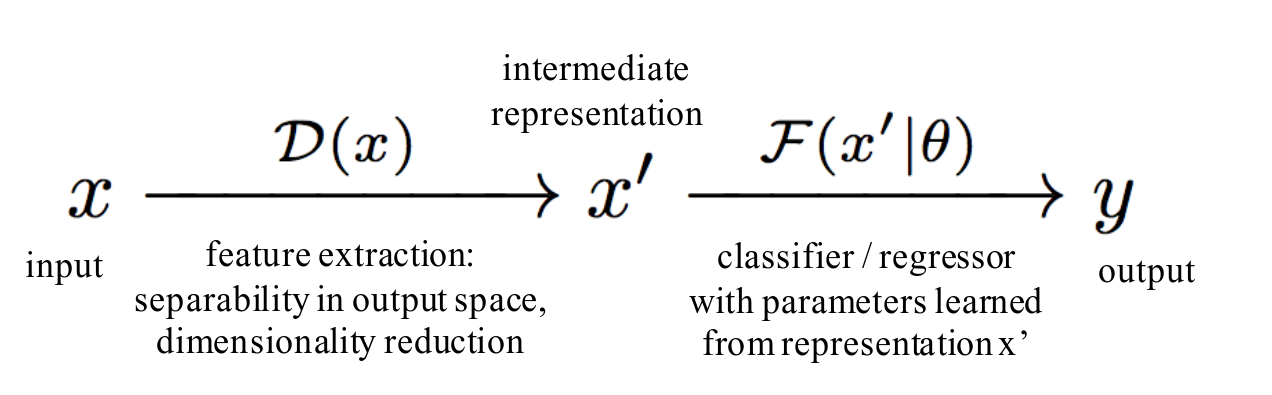
\includegraphics[width=0.9\linewidth]{images/ml.png}  
    \caption{Traditional Supervised learning}
  \end{figure}
\end{frame}


\begin{frame}{Deep Learning (Supervised)}
 \begin{figure}[h]
    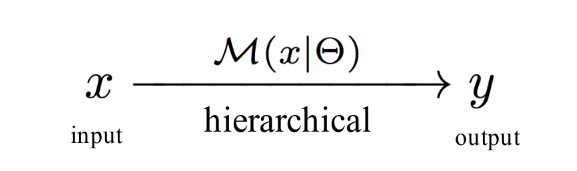
\includegraphics[width=0.9\linewidth]{images/dl.png}  
    \caption{Deep learning}
  \end{figure}
 \begin{itemize}
  \item<+-> Hierarchical representations of features.
  \item<+-> Joint learning of representation.
  \item<+-> Increased levels of abstraction.
 \end{itemize}
\end{frame}

\begin{frame}{Perceptron}
 \begin{figure}[h]
    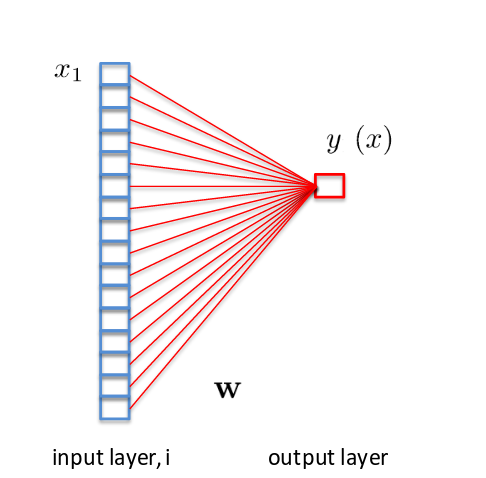
\includegraphics[width=0.5\linewidth]{images/perceptron.png}  
    \caption{A perceptron (close to a biological neuron)}
  \end{figure}
  $$ y(x) = f( W^T x )$$
\end{frame}

\begin{frame}{Logistic Regression}
 \begin{figure}[h]
    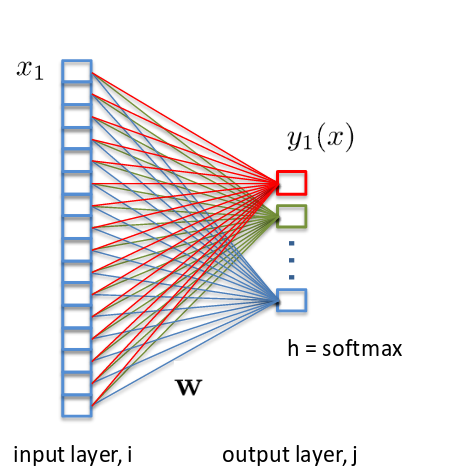
\includegraphics[width=0.5\linewidth]{images/lr.png}  
    \caption{A perceptron (A collection of perceptrons)}
  \end{figure}
\end{frame}

\begin{frame}{Logistic Regression}
Binary classification:
$$P(y = 1 | x) = h_w(x) = \frac{1}{1 + exp(-W^T x)}$$
$$P(y = 0 | x) = 1 - h_w(x) = 1 - P(y = 1 | x)$$
\end{frame}

\begin{frame}{Logistic Regression}
 Cost function: 
 $$ J(w) = - \sum_{i} ( y^i log(h_w(x^i)) + (1 - y^i) log(1 - h_w(x^i))  ) $$
 Learning Weights : Gradient Descent
 $$\nabla_w J(w) = \frac{\partial J(w)}{\partial w_j} = \sum_i x^i_j (h_w(x^i) - y^i) $$
\end{frame}

\begin{frame}{Gradient Descent}
\begin{figure}[h]
    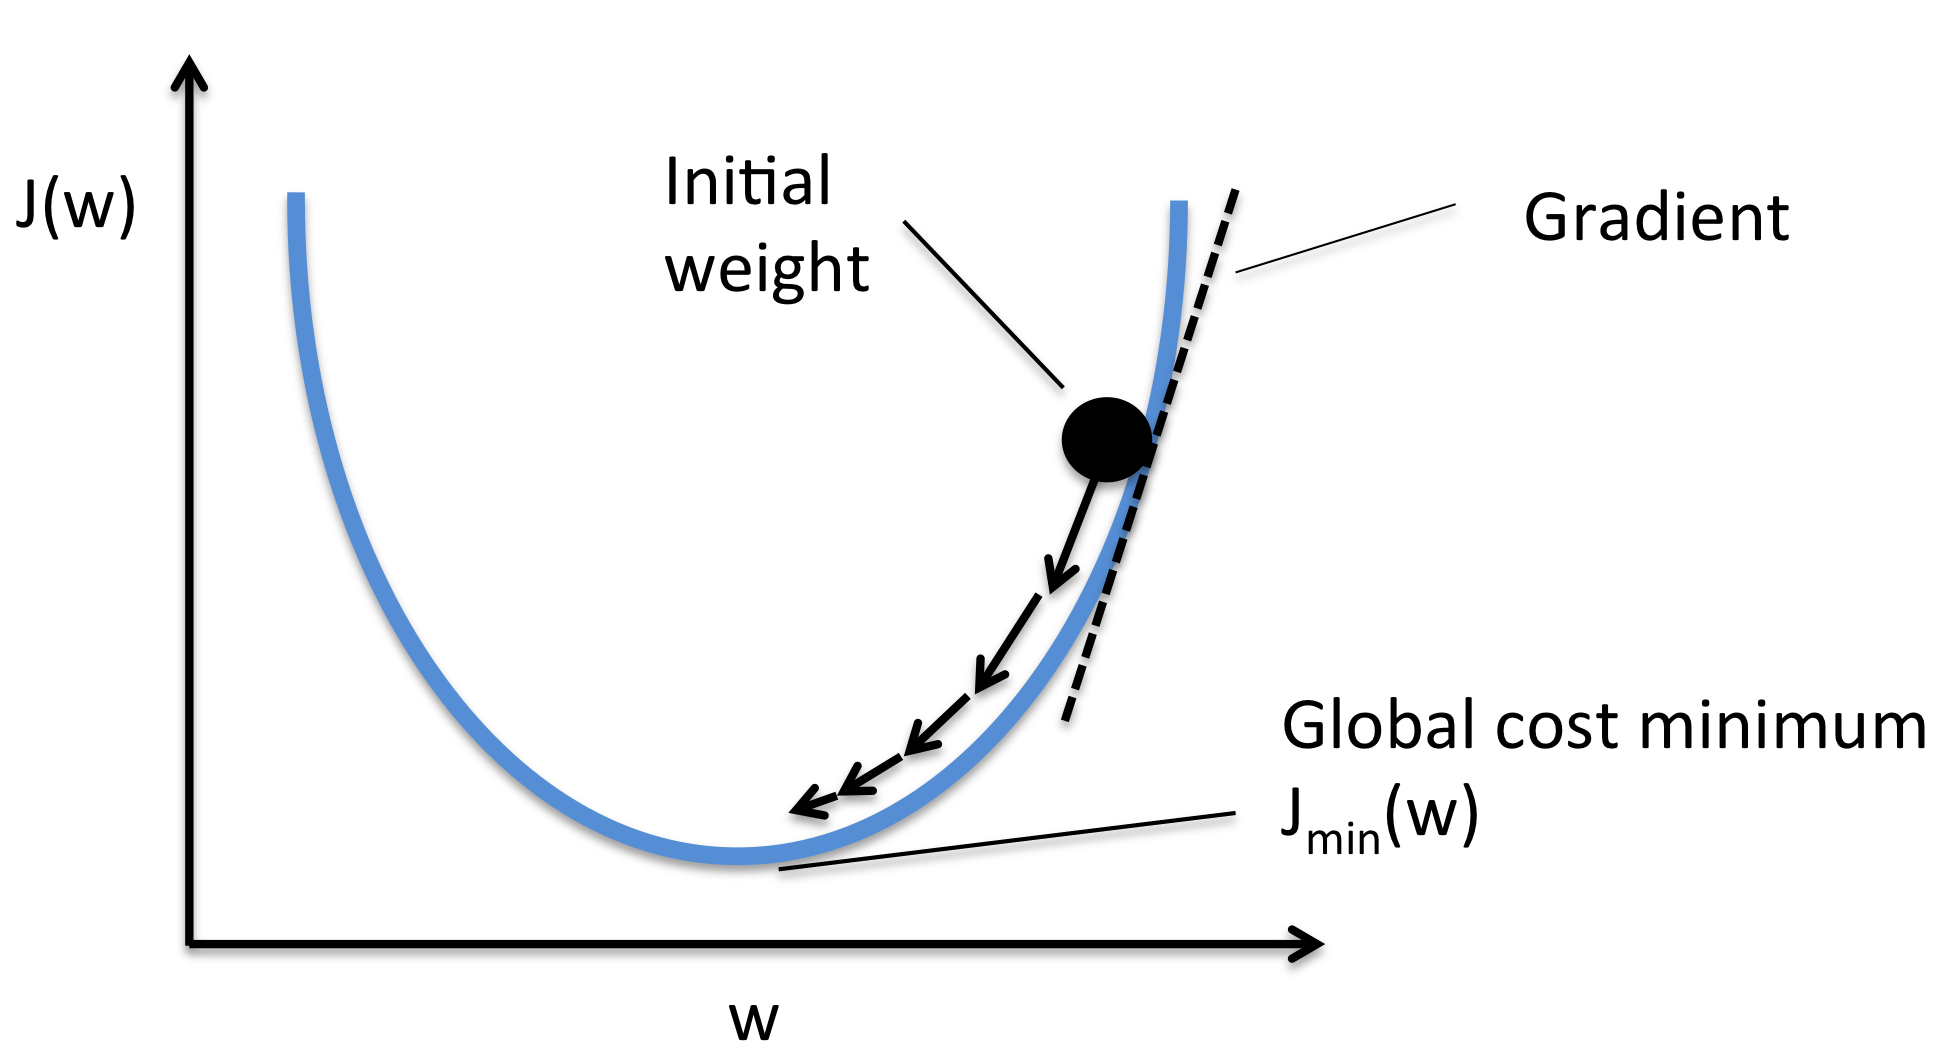
\includegraphics[width=0.7\linewidth]{images/gd.png}  
    \caption{Update weights in the direction of negative gradient.}
  \end{figure}
\end{frame}

\begin{frame}{Multi Layer Perceptron}
\begin{figure}[h]
    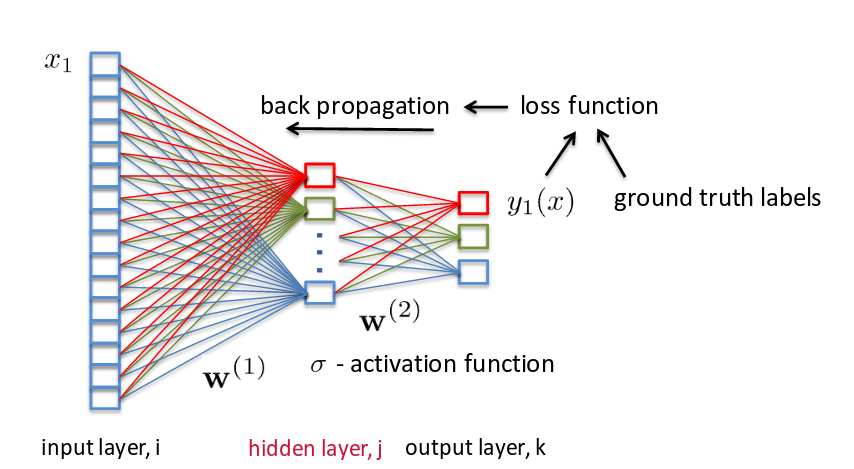
\includegraphics[width=0.7\linewidth]{images/mlp.png}  
    \caption{Multiple layers of perceptron}
  \end{figure}
  Learning weights: Same as before but apply chain rule.
  $$ \frac{\partial x}{\partial y}  = \frac{\partial x}{\partial z} * \frac{\partial z}{\partial y} $$
\end{frame}

\begin{frame}{Deep Neural Networks}
 \begin{figure}[h]
    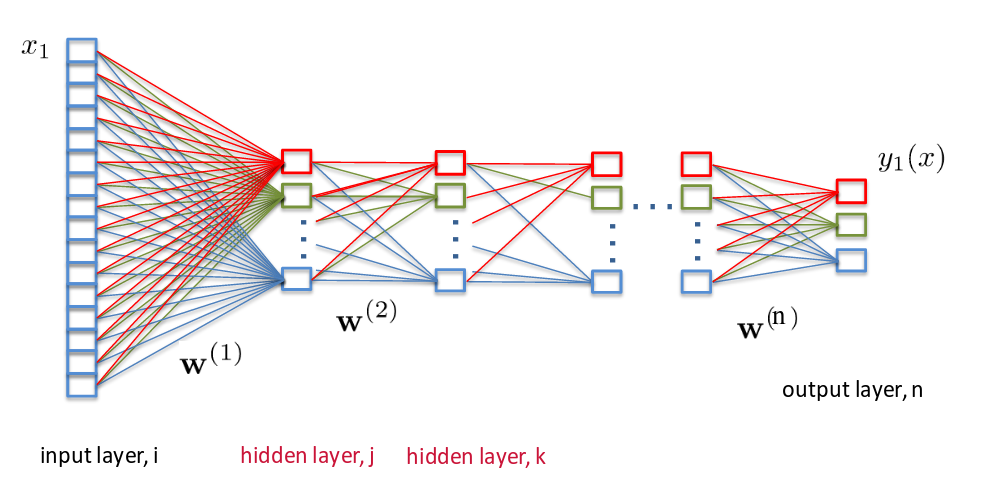
\includegraphics[width=0.7\linewidth]{images/dnn.png}  
    \caption{Deep Neural Networks}
  \end{figure}
  \begin{itemize}
   \item<+-> Simply adding layers won't work.
   \item<+-> Too many parameters to train.
   \item<+-> Need smart architectures to capture additional priors.
   \item<+-> Two most commonly used architectures are CNNs and RNNs.
  \end{itemize}
\end{frame}

\begin{frame}{Convolutional Neural Networks}
\begin{figure}[h]
    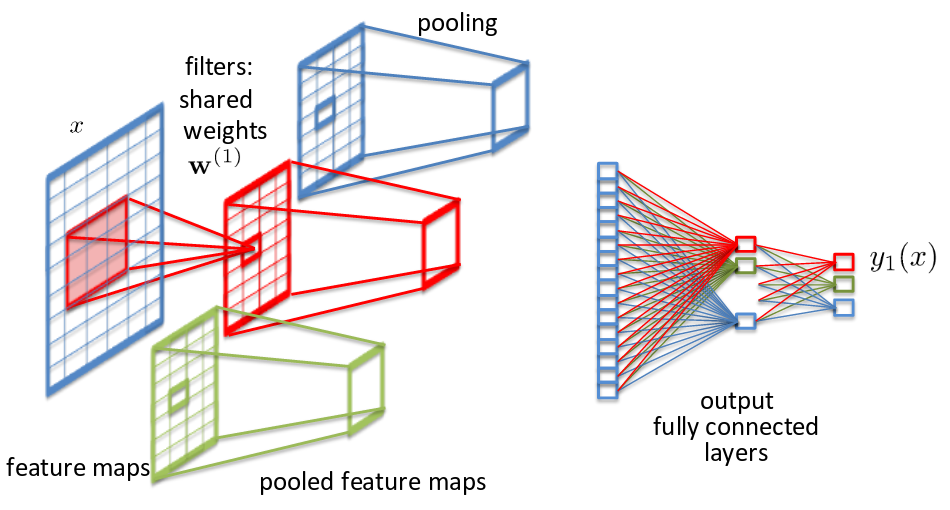
\includegraphics[width=0.7\linewidth]{images/cnn.png}  
    \caption{Convolutional Neural Networks}
  \end{figure}
\begin{itemize}
\item<+-> Each layers learns a set of convolution kernels.
\item<+-> Captures a very important prior --smoothness prior-- known to computer vision community for a very long time.
\item<+-> Much less number of parameters.
\end{itemize}
\end{frame}

\begin{frame}{Recurrent Neural Networks}
\begin{figure}[h]
    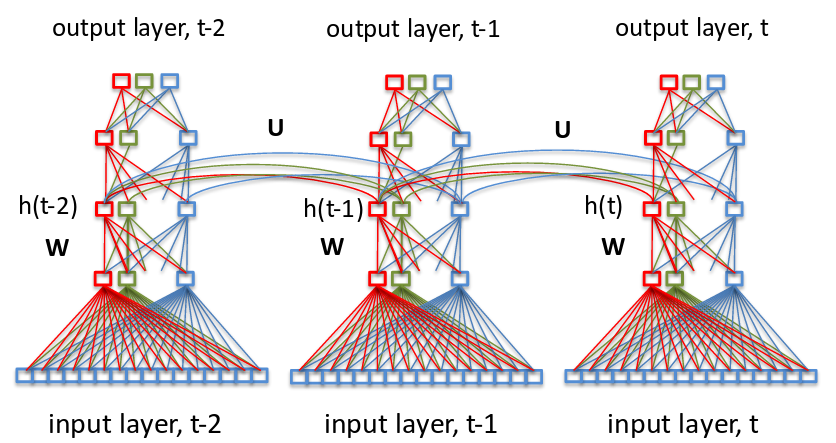
\includegraphics[width=0.7\linewidth]{images/rnn.png}  
    \caption{Recurrent Neural Networks}
  \end{figure}
  
\begin{itemize}
\item<+-> Used for predicting sequential data 
\item<+-> Captures dependences across time frames.
\item<+-> Usually harder to train (Vanishing Gradients).
\end{itemize}

\end{frame}


\begin{frame}{LSTM}
 \begin{figure}[h]
    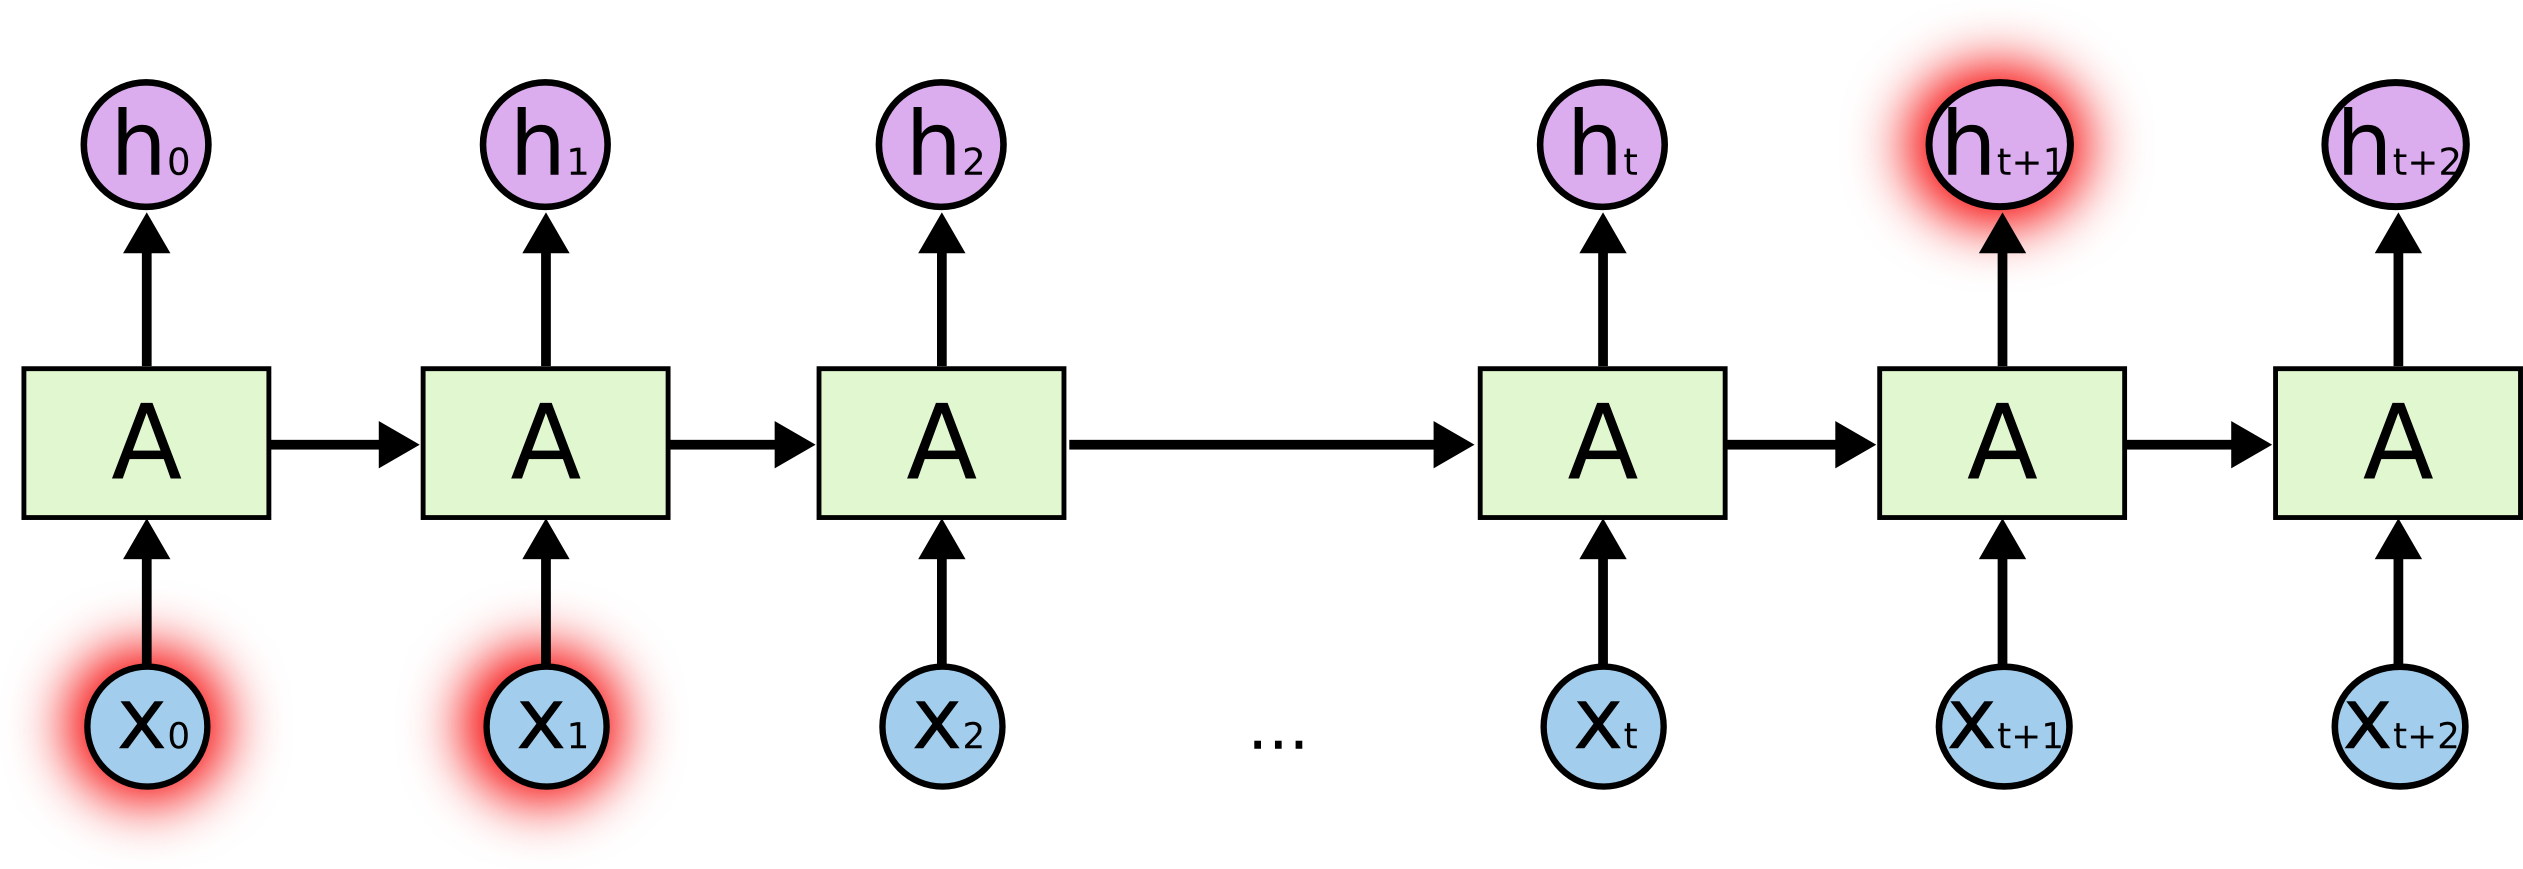
\includegraphics[width=0.4\linewidth]{images/rnn_n.png}  
    \caption{Recurrent Neural Networks}
  \end{figure}
   \begin{figure}[h]
    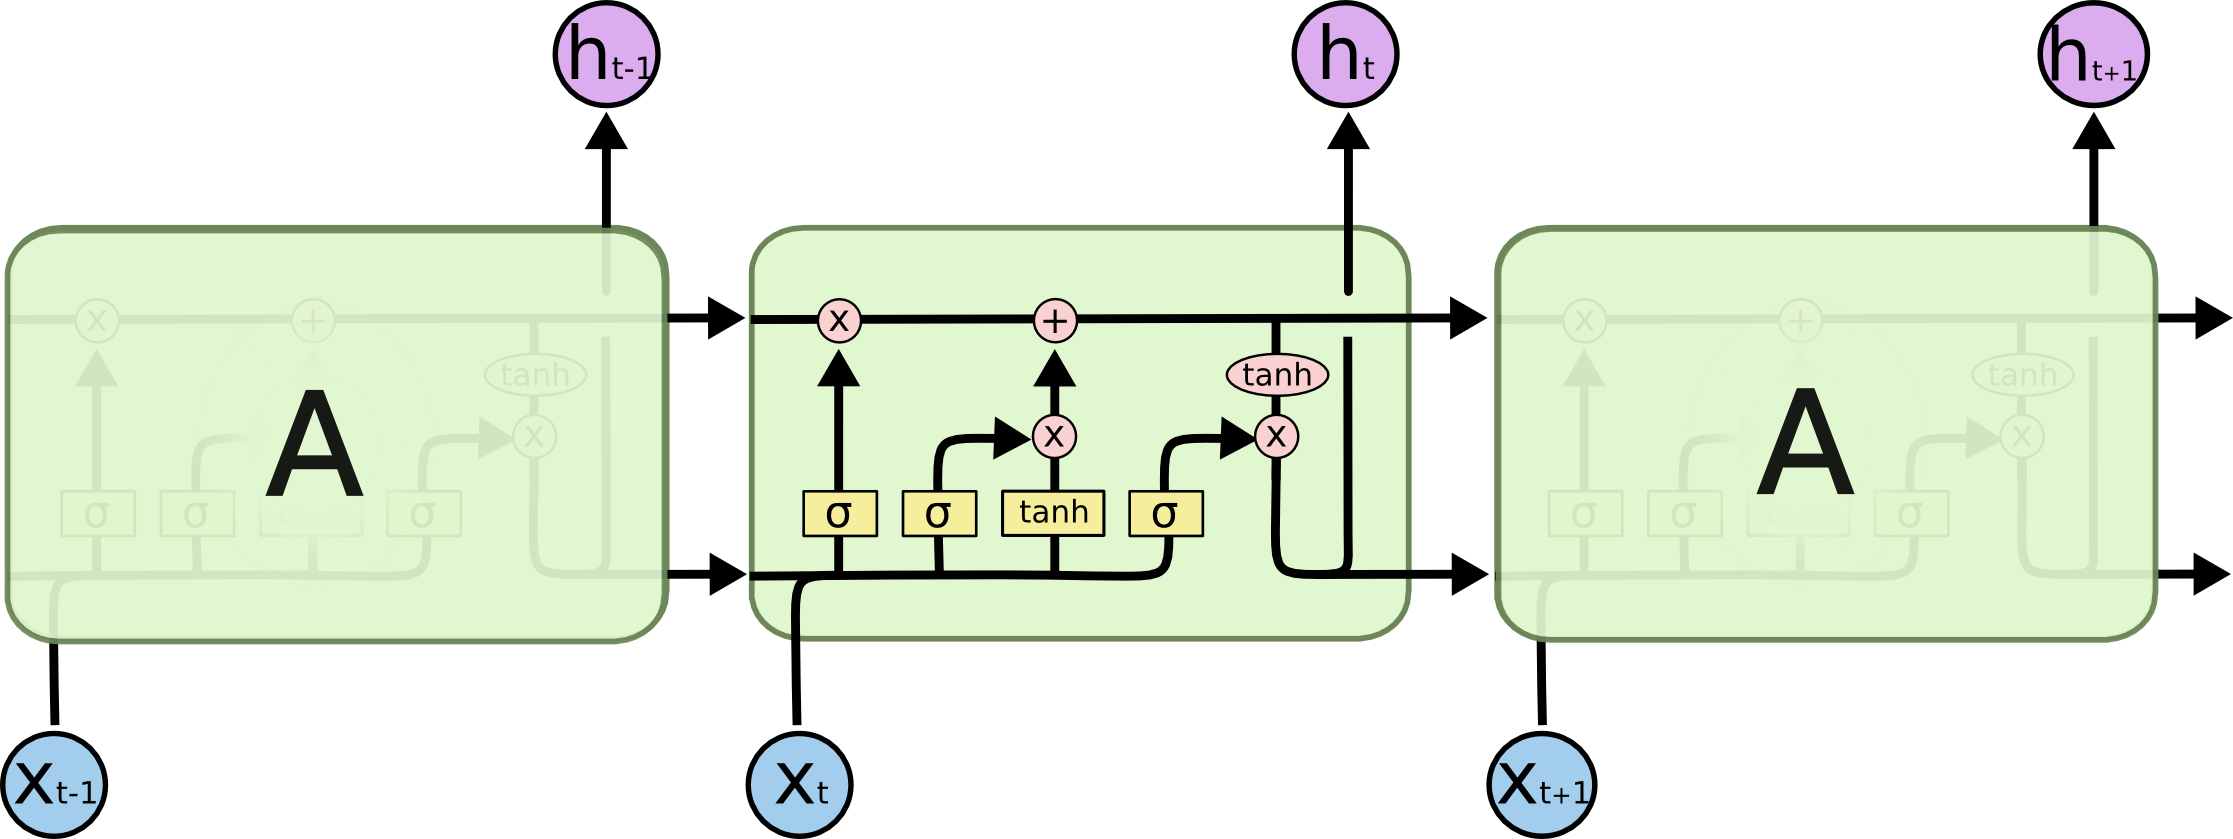
\includegraphics[width=0.6\linewidth]{images/lstm.png}  
    \caption{Long Short Term Memory}
  \end{figure}
\end{frame}


\begin{frame}{LSTM}
 \begin{figure}[h]
    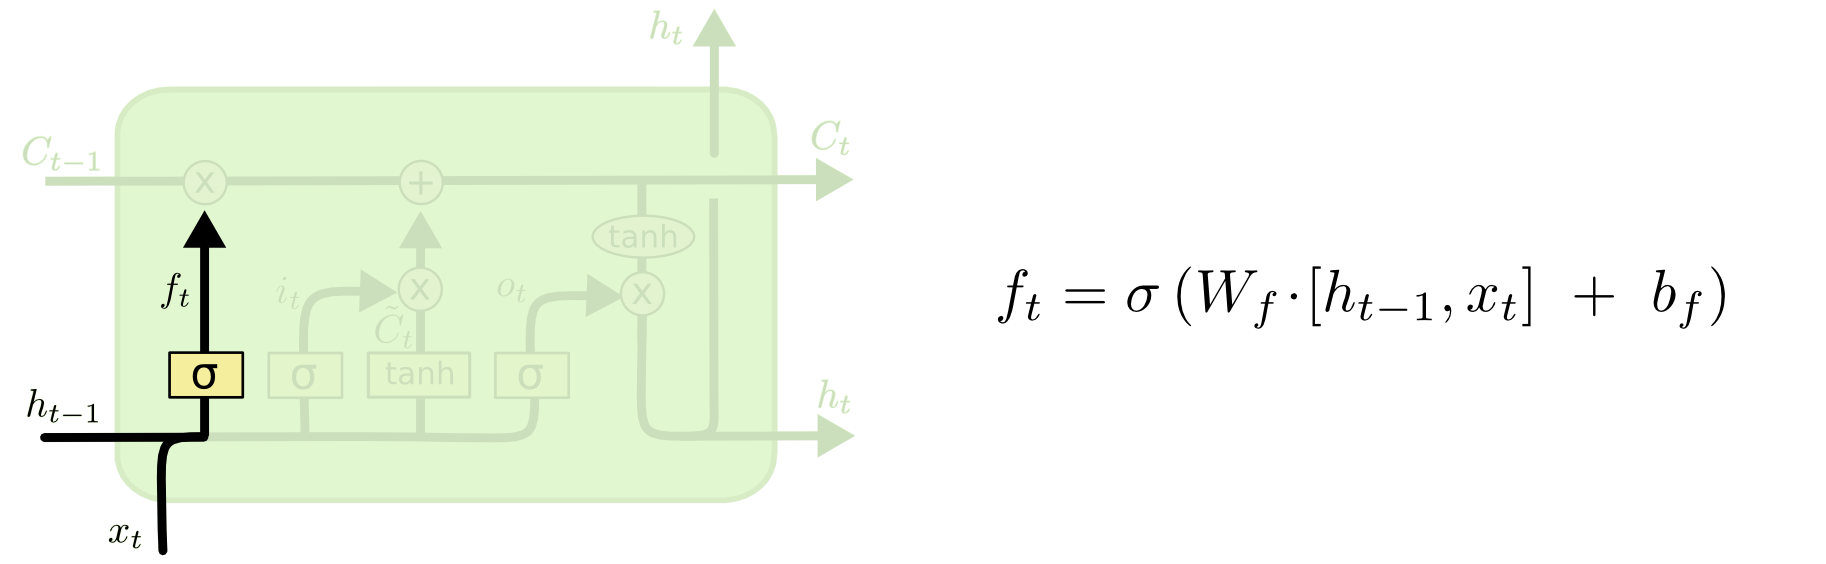
\includegraphics[width=0.6\linewidth]{images/lstm_forget.png}  
    \caption{LSTM Forget gate}
  \end{figure}
   \begin{figure}[h]
    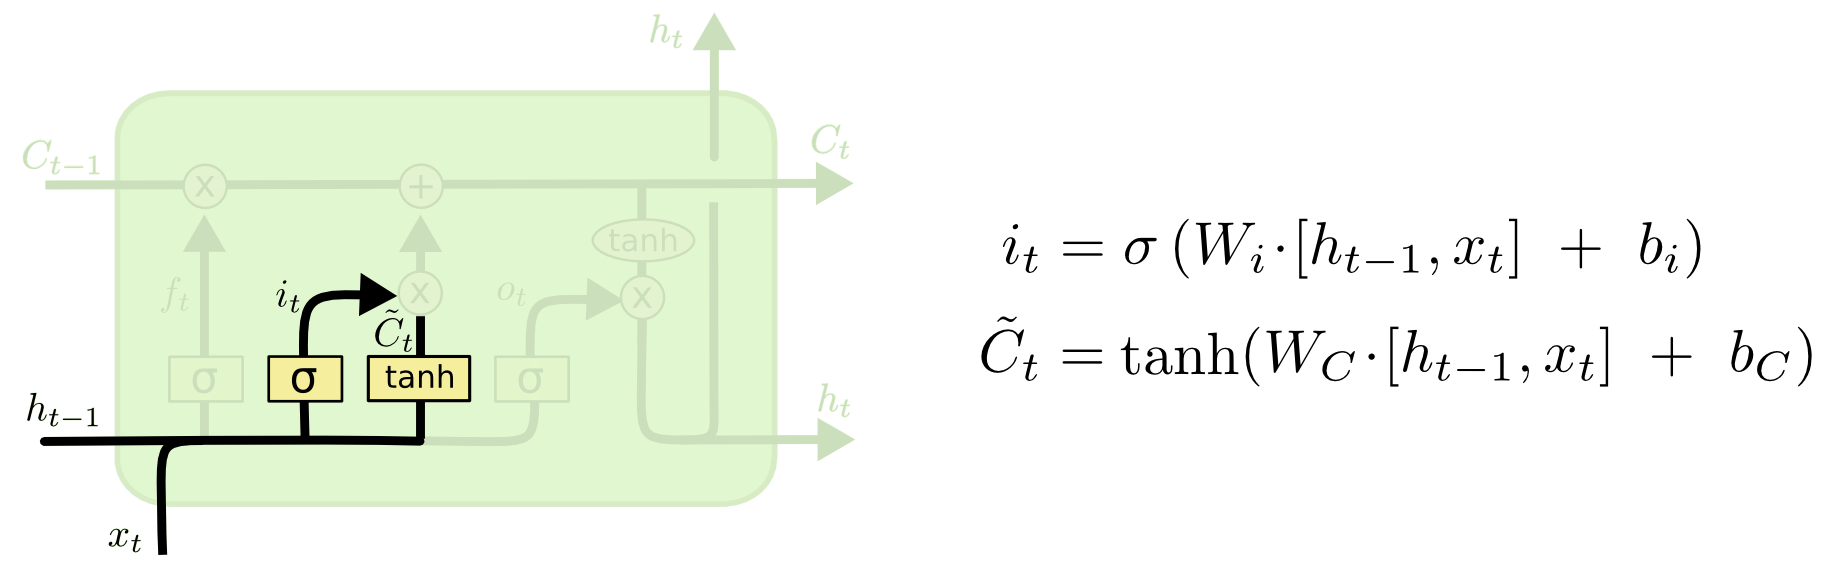
\includegraphics[width=0.6\linewidth]{images/lstm_add.png}  
    \caption{LSTM new content}
  \end{figure}
\end{frame}


\begin{frame}{LSTM}
 \begin{figure}[h]
    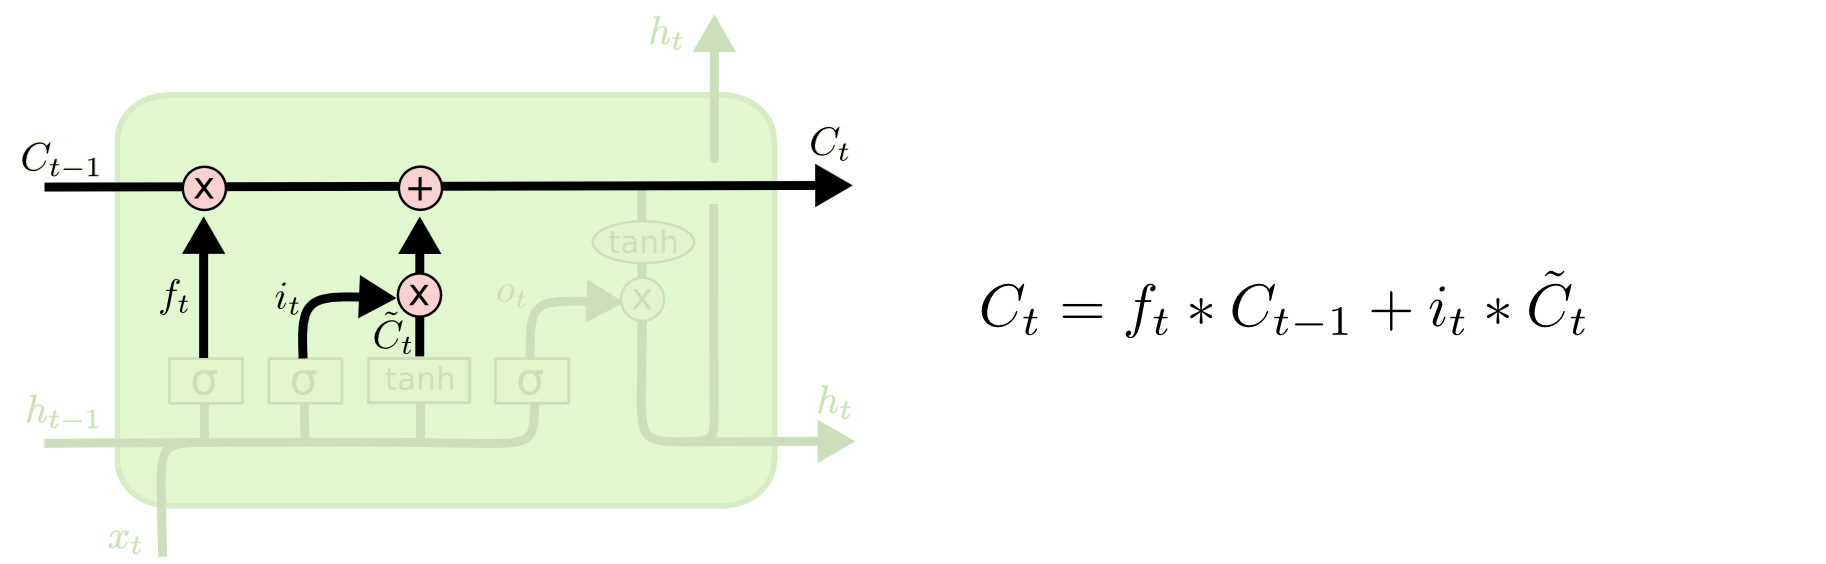
\includegraphics[width=0.6\linewidth]{images/lstm_add1.png}  
    \caption{LSTM Add gate}
  \end{figure}
   \begin{figure}[h]
    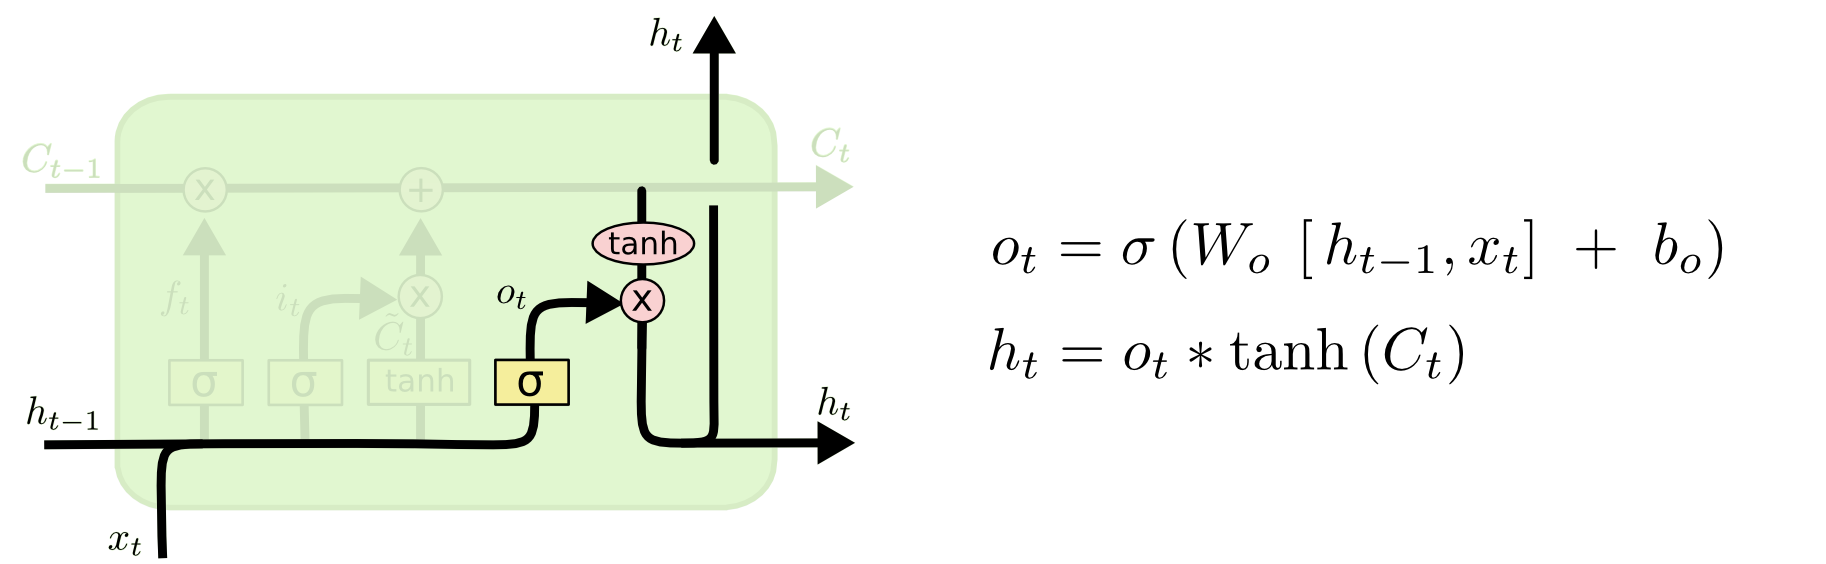
\includegraphics[width=0.6\linewidth]{images/lstm_output.png}  
    \caption{LSTM Output Gate}
  \end{figure}
\end{frame}


\begin{section}{Neural Machine Translation}
\end{section}

\begin{frame}{Neural Machine Translation}
 $$ arg\,max _{y}  \,\, p(x|y)$$
 In Neural Machine Translation, a parameterized model (a neural network) is trained to maximize the conditional probability of the sentence pairs given parallel training corpus.
\end{frame}

\begin{frame}{NMT - A historic perspective}
  \begin{figure}[h]
    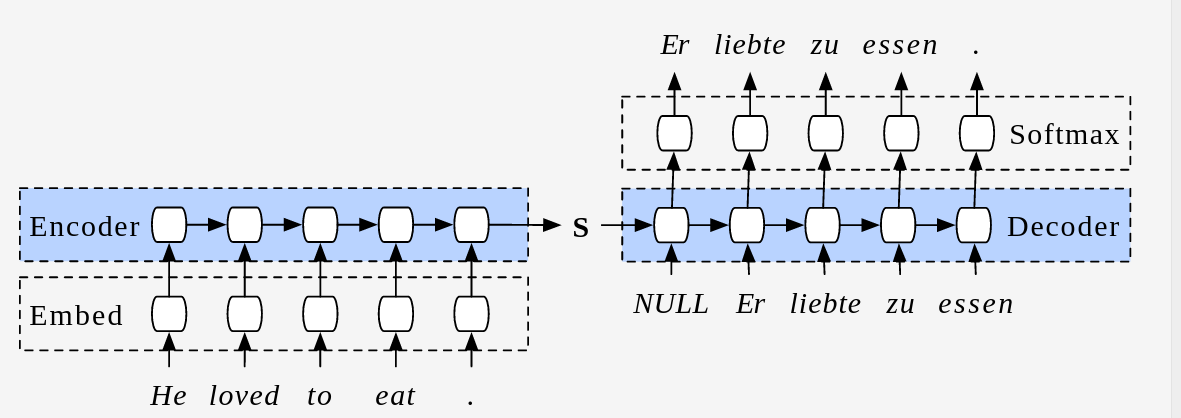
\includegraphics[width=0.9\linewidth]{images/enc_dec.png}  
    \caption{Encoder-Decoder model for Machine Translation}
  \end{figure}
\begin{itemize}
 \item<+-> Fixed size encodings.
 \item<+-> Each language typically required an Encoder and Decoder.
\end{itemize}
\end{frame}

\begin{section}{Jointly learning to Align and translate}
\end{section}
\begin{frame}{Jointly learning to Align and translate}
\begin{figure}[h]
    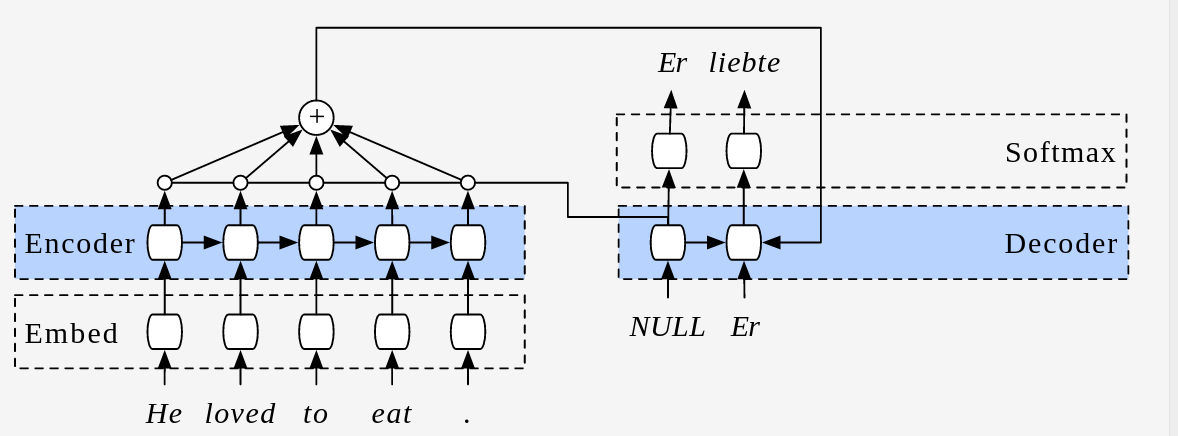
\includegraphics[width=0.9\linewidth]{images/context.png}  
    \caption{Encoder-Decoder model with context}
  \end{figure}
\end{frame}

\begin{frame}{Jointly learning to Align and translate}
For a input sentence, $X = (x_1,\cdots, x_{T_{x}} )$. The NMT \footfullcite{NEURAL MACHINE TRANSLATION BY JOINTLY LEARNING TO ALIGN AND TRANSLATE. Dzmitry Bahdanau, KyungHyun Cho, Yoshua Bengio, ICLR, 2015}
system consists of,
  \begin{itemize}
   \item<+-> Encoder and Decoder are multi-layer recurrent neural networks (RNNs).
   \item<+-> Encoder RNN, at each input step t, generates hidden state, $h_t = f(x_t, h_{t-1})$.
   \item<+-> Context vector encodes the input sequence as, $c = q(\{h_1,\cdots,h_{T_x}\})$.
  \end{itemize}
\end{frame}

\begin{frame}{Jointly learning to Align and translate}
\begin{itemize}
 \item The decoder is trained to predict the next work $y_t$ given the context vector $c$ and all previously predicted words $\{ y_1, \cdots, y_{t-1}\}$
 $$ p(y) = \prod^{T}_{t=1} p(y_t | \{ y_1, \cdots, y_{t-1}\} ,c ) $$
 \item With RNN, each conditional probability is modeled as,
 $$ p(y_t | \{ y_1, \cdots, y_{t-1}\}, c) = g(y_{t-1}, s_t, c) $$ where $s_t$ is the hidden state of the RNN.
 \end{itemize}

\end{frame}


\begin{frame}{Context Vector}
  The context vector for a input sentence $i$, is computed as a weighted sum of hidden states of the encoder (also known as \textbf{annotations})
  $$ c_i = \sum_{j=1}^{T_{x}} \alpha_{ij} h_j$$
  $$ \alpha_{ij} = \frac{ exp(e_{ij})}{ \sum_{k=1}^{T_x} exp (e_{ik})}$$

where,
$$ e_{ij} = a(s_{i-1}, h_j)  $$ is the alignment model that scores how well the inputs around the $j$ and the output at the position $i$ match.

A feedforward neural network is used as the alignment model and is \textbf{jointly trained} with all the NMT system as a whole.
\end{frame}

\begin{frame}{Visualization of the context}
 \begin{figure}[h]
    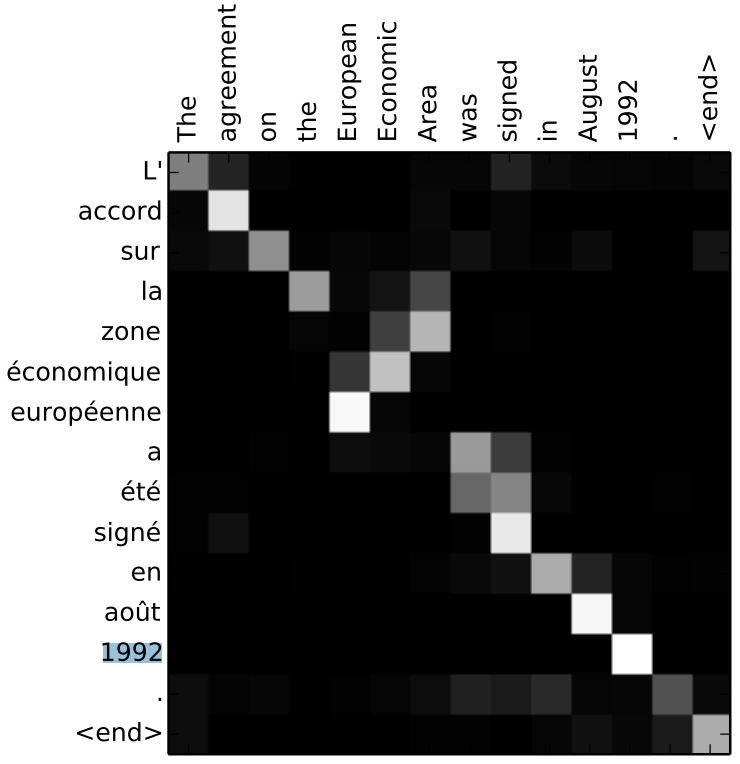
\includegraphics[height=8cm]{images/contextres.png}  
    \caption{Visualization of the context in action}
  \end{figure}
\end{frame}

\begin{frame}{Bi-directional Encoder}
 
 \begin{figure}[h]
    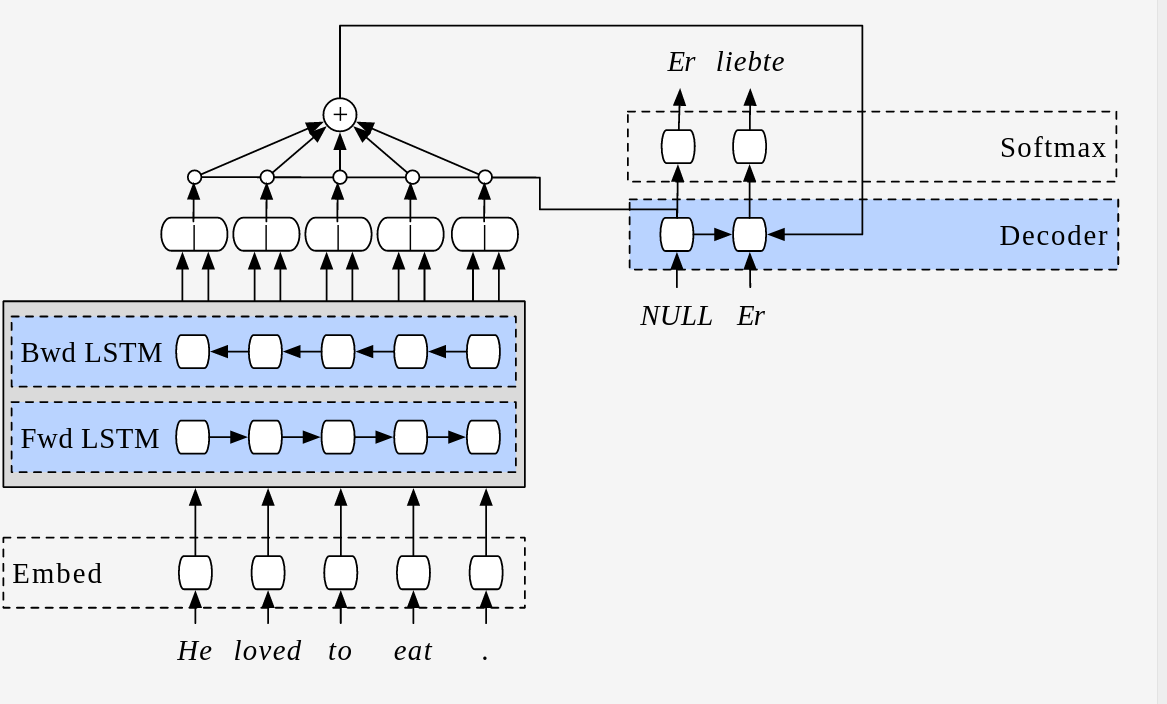
\includegraphics[width=0.9\linewidth]{images/birnn.png}  
    \caption{Bi-directional Encoder}
  \end{figure}
  \begin{itemize}
   \item<+-> Recurrent connection in both directions.
   \item<+-> Two independent states, updated independently.
  \end{itemize}
\end{frame}


\begin{section}{Seq2Seq Learning}
\end{section}

\begin{frame}{Seq2Seq Learning}
 Machine Translation is can treated as a special case of a more generic sequence to sequence modeling.
 \begin{enumerate}
  \item<+-> Idea is simple: Throw more power at the network.
  \item<+-> Deep LSTM layers.
  \item<+-> No special handling for Machine translation.
  \item<+-> Trained with SGD.
 \end{enumerate}
$$ p(y_1, \cdots, y_T| x_1, \cdots, x_T) = \prod_{t=1}^{T} p(y_t| v, y_1, \cdots, y_{t-1})$$
\end{frame}


\begin{frame}{Seq2Seq Learning}
 \begin{figure}
    \centering
    \begin{tabular}{cc}
	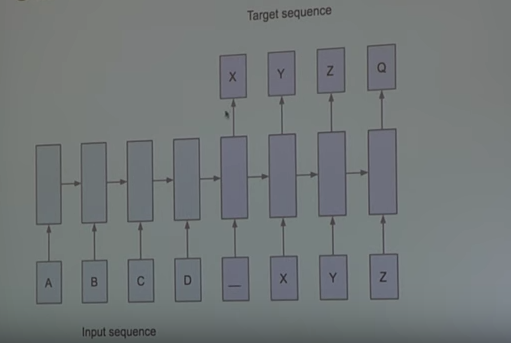
\includegraphics[width=.49\linewidth]{images/seq2seq.png} &
	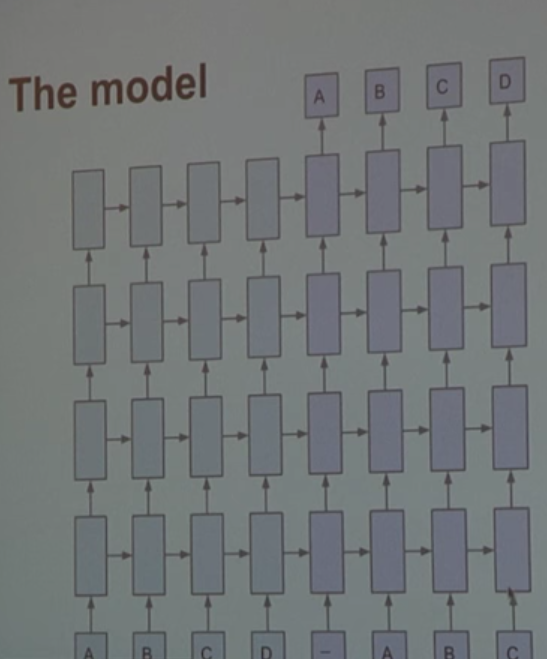
\includegraphics[width=.49\linewidth]{images/seq2seqDeep.png} \\
	\footnotesize(a) Seq2Seq model & \footnotesize(b) More powerful model \\
    \end{tabular}
    \end{figure}
\end{frame}

\begin{frame}{Seq2Seq Learning}
\begin{itemize}
 \item<+->  Trained in WMT English to French dataset with 12M sentences consisting of 348M French words and 304M English words.
 \item<+->  Used 160,000 of the most frequent words for the source language and 80,000 of the most frequent words for the target language
 \item<+->  Every out-of-vocabulary word was replaced with a special “UNK” token
\end{itemize}
\end{frame}

\begin{frame}{Seq2Seq Learning}
 Architecture details:
\begin{itemize}
 \item<+->  4 LSTM layers.
 \item<+->  1000 LSTM cells in each layer.
 \item<+->  1000 dimensional word embeddings.
 \item<+->  Achieved BLEU score of 33.3 on WMT’14 English-to-French dataset.
\end{itemize}
\end{frame}


\begin{section}{Google NMT}
\end{section}

\begin{frame}{Google NMT}
\begin{itemize}
 \item<+-> Paper describing all the details about the Google's MT system.
 \item<+-> Heavily borrows from the previous two papers.
 \item<+-> Also, adds almost all the nice ideas in Deep learning research in the last few years.
 \item<+-> Not just a research idea but already serves billions of queries a day.
\end{itemize}
\end{frame}


\begin{frame}{Google NMT}
 \begin{figure}[h]
    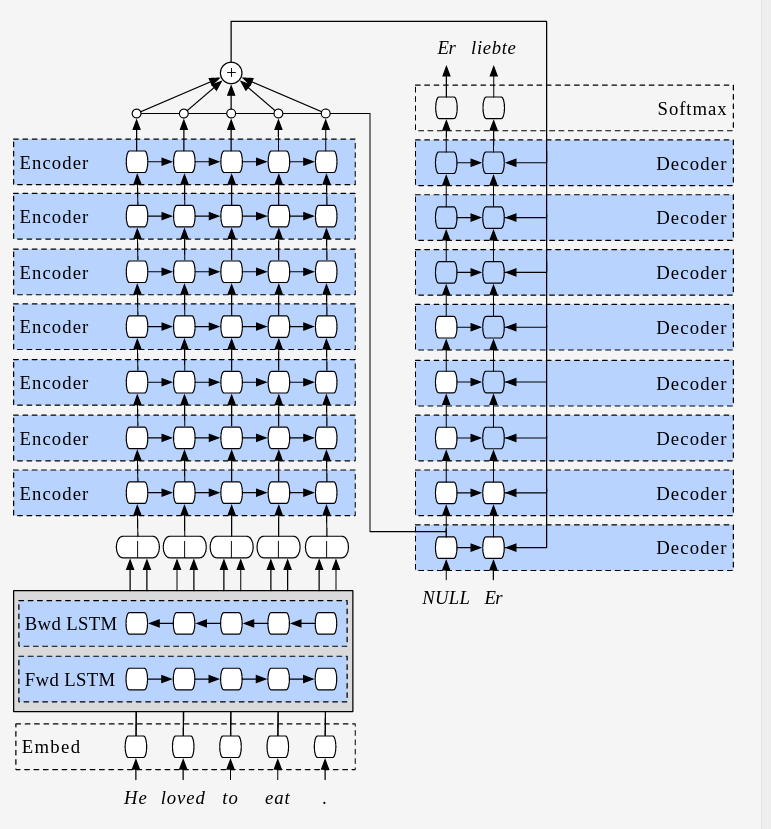
\includegraphics[height=7.5cm]{images/gnmt_1.png}  
    \caption{Simple Encoder-Decoder but more deeper as in Seq2Seq, and Context}
  \end{figure}
\end{frame}



\begin{frame}{Residual learning}
  \begin{figure}[h]
    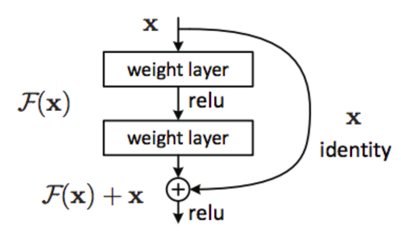
\includegraphics[width=.9\linewidth]{images/residual.png}  
    \caption{ Residual networks}
  \end{figure}
  \vspace{-1cm}
  Residual connections enables training of very deep networks. \footfullcite{Deep Residual Learning for Image Recognition. Kaiming He, Xiangyu	Zhang, Shaoqing	 Ren, & Jian Sun. CVPR, 2016}
\end{frame}

\begin{frame}{Google NMT with Residual connection}
 \begin{figure}[h]
    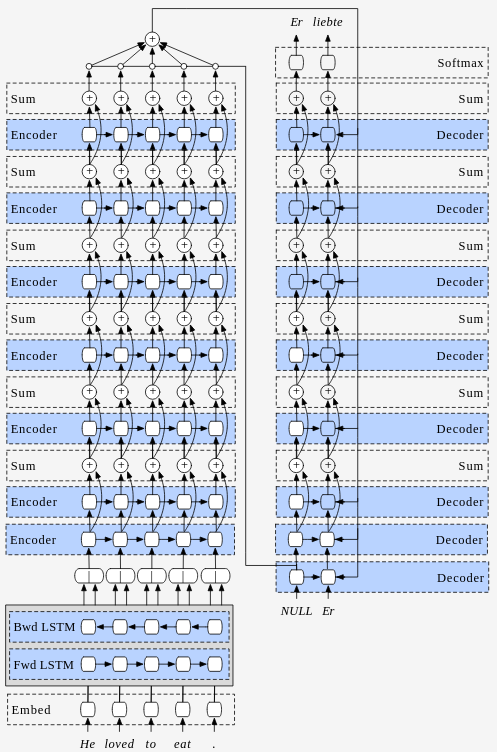
\includegraphics[height=7.5cm]{images/residual_gnmt.png}  
    \caption{ GNMT with residual connections.}
  \end{figure}
\end{frame}

\begin{frame}{Google NMT}
\textbf{Google NMT properties}
\begin{itemize}
 \item<+-> Achieved a BLEU score of 38.95 BLEU on WMT’14 English-to-French dataset. 
 \item<+-> One Encoder and one Decoder for all the languages.
 \item<+-> This joint training of languages improves accuracy for languages for which not much training data exist.
 \item<+-> The input language are encoded using word2vec for all languages.
 \item<+-> One additional token $(<\_\_EN\_\_>, <\_\_FR\_\_>, <\_\_DE\_\_>, <\_\_ES\_\_>)$ indicating the target language to be generated.
 \item<+-> One giant model that runs all Google translate queries.
\end{itemize}
\end{frame}

\begin{frame}{Conclusion}
\textbf{Neural Machine Translation systems,}
\begin{itemize} 
 \item Are State-of-the-art in machine translation.
 \item Greatly benefited from the neural network research by other communities.
 \item Used in production by companies like Google, Microsoft, Facebook, etc.
\end{itemize}
\end{frame}

\begin{frame}{Conclusion}
 \begin{itemize}
  \item<+-> Actually, I lied to you all.
  \item<+-> Maybe, we don't need such a complex network like GNMT to achieve better results.
  \item<+-> \textquotedblleft Attention Is All You Need\textquotedblright arxiv preprint from Google threw away all LSTMS, Residual connections, etc., but managed to achieve BLEU score of 41.0 with  \textcolor{red} {only feedforward connections and attention.}
 \end{itemize}

\end{frame}


\end{document}